\documentclass[fontsize=10pt]{article}
\usepackage[utf8]{inputenc}
\usepackage[T1]{fontenc}
\usepackage{graphicx} % handles figures
\usepackage[fleqn]{mathtools}
\usepackage{amsmath}
\usepackage{hyperref}
\usepackage{amssymb}
\usepackage{xcolor}

%Insertion de tout un tas de librairie qui nous seront probablement inutiles pour la pluspart mais it's always good to have them
\title{\textbf{Maths Discrètes}\\ Solutions TP 5}
\date{}
\begin{document}
\maketitle % fais le titre écris plus haut


\section*{Exercice 1}
$G_1$ possède un chemin d'Euler.\\
$G_2$ possède un chemin d'Euler.\\
$G_3$ ne possède pas de chemin d'Euler.

\section*{Exercice 2}
\begin{enumerate}
\item Pour tout n impair, $K_n$ aura un degré $n-1$ pair
\item Pour n = 2, puisque tout n impair est un circuit et $n>2$ pair n'a pas de chemins et $n=1$
\end{enumerate}

\section*{Exercice 3}

Sachant qu'un circuit existe depuis $v$, $u \rightarrow v$ et $v \rightarrow u$ sont possibles, donc $u \rightarrow u$ est un circuit.

\section*{Exercice 4}
$m$ et $n$ pairs
\newpage
\section*{Exercice 5}
Un graphe dirigé est faiblement connexe s'il existe un chemin entre deux sommets quelquonques du graphe sous-jacent.\\
\textit{Fun fact, on a un bonus en info: il doit exister un chemin vers tous les autres noeuds depuis au moins un sommet, sans pour autant être fortement connexe. En respectant ce point, on a juste moins de choix.} 
\begin{figure}[hbtp]
\centering
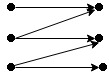
\includegraphics[scale=0.2]{TP5Exo5.jpg}
\end{figure}

\section*{Exercice 6}

\begin{figure}[hbtp]
\centering
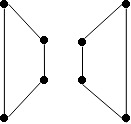
\includegraphics[scale=1]{TP5Exo6.jpg}
\end{figure}





























\end{document}
